\documentclass[]{article}
\usepackage{lmodern}
\usepackage{amssymb,amsmath}
\usepackage{ifxetex,ifluatex}
\usepackage{fixltx2e} % provides \textsubscript
\ifnum 0\ifxetex 1\fi\ifluatex 1\fi=0 % if pdftex
  \usepackage[T1]{fontenc}
  \usepackage[utf8]{inputenc}
\else % if luatex or xelatex
  \ifxetex
    \usepackage{mathspec}
  \else
    \usepackage{fontspec}
  \fi
  \defaultfontfeatures{Ligatures=TeX,Scale=MatchLowercase}
\fi
% use upquote if available, for straight quotes in verbatim environments
\IfFileExists{upquote.sty}{\usepackage{upquote}}{}
% use microtype if available
\IfFileExists{microtype.sty}{%
\usepackage{microtype}
\UseMicrotypeSet[protrusion]{basicmath} % disable protrusion for tt fonts
}{}
\usepackage[margin=1in]{geometry}
\usepackage{hyperref}
\hypersetup{unicode=true,
            pdfborder={0 0 0},
            breaklinks=true}
\urlstyle{same}  % don't use monospace font for urls
\usepackage{graphicx,grffile}
\makeatletter
\def\maxwidth{\ifdim\Gin@nat@width>\linewidth\linewidth\else\Gin@nat@width\fi}
\def\maxheight{\ifdim\Gin@nat@height>\textheight\textheight\else\Gin@nat@height\fi}
\makeatother
% Scale images if necessary, so that they will not overflow the page
% margins by default, and it is still possible to overwrite the defaults
% using explicit options in \includegraphics[width, height, ...]{}
\setkeys{Gin}{width=\maxwidth,height=\maxheight,keepaspectratio}
\IfFileExists{parskip.sty}{%
\usepackage{parskip}
}{% else
\setlength{\parindent}{0pt}
\setlength{\parskip}{6pt plus 2pt minus 1pt}
}
\setlength{\emergencystretch}{3em}  % prevent overfull lines
\providecommand{\tightlist}{%
  \setlength{\itemsep}{0pt}\setlength{\parskip}{0pt}}
\setcounter{secnumdepth}{0}
% Redefines (sub)paragraphs to behave more like sections
\ifx\paragraph\undefined\else
\let\oldparagraph\paragraph
\renewcommand{\paragraph}[1]{\oldparagraph{#1}\mbox{}}
\fi
\ifx\subparagraph\undefined\else
\let\oldsubparagraph\subparagraph
\renewcommand{\subparagraph}[1]{\oldsubparagraph{#1}\mbox{}}
\fi

%%% Use protect on footnotes to avoid problems with footnotes in titles
\let\rmarkdownfootnote\footnote%
\def\footnote{\protect\rmarkdownfootnote}

%%% Change title format to be more compact
\usepackage{titling}

% Create subtitle command for use in maketitle
\providecommand{\subtitle}[1]{
  \posttitle{
    \begin{center}\large#1\end{center}
    }
}

\setlength{\droptitle}{-2em}

  \title{}
    \pretitle{\vspace{\droptitle}}
  \posttitle{}
    \author{}
    \preauthor{}\postauthor{}
    \date{}
    \predate{}\postdate{}
  
\pagestyle{empty}
\usepackage{graphicx}
\usepackage{epstopdf}
\textbackslash{}DeclareGraphicsRule\{.tif\}\{png\}\{.png\}\{`convert
\usepackage{color}
\usepackage{hyperref}
\usepackage{amssymb}
\usepackage{algpseudocode}

\begin{document}

\textbackslash{}begin\{document\} \thispagestyle{empty}
\includegraphics{../../../psulogo_horiz_bw.eps}\hfill\includegraphics{../../../deptlogo}

\hypertarget{section}{%
\section{}\label{section}}

STAT 572

\hypertarget{hw1}{%
\subsection{HW1}\label{hw1}}

\hypertarget{a-exponential-case}{%
\subsubsection{1 A Exponential Case}\label{a-exponential-case}}

We write \(Y\sim Exp(\theta)\) to indicate that Y has the Exponential
distribution, that is, its p.d.f. is

\(p(y|\theta) = Exp(y|\theta) = \theta e^{-\theta y}1_{\{y>0\}}\)

The Exponential distribution has some special properties that make it a
good model for certain applications. It has been used to model the time
between events (such as neuron spikes, website hits, neutrinos captured
in a detector), extreme values such as maximum daily rainfall over a
period of one year, or the amount of time until a product fails
(lightbulbs are a standard example). Suppose you have data
\(y_1,...,y_n\) which you are modeling as iid observations from an
Exponential distribution, and suppose that your prior is
\(\theta\sim Gamma(a,b)\), defined as in the previous question.

(a). Derive the formula for the posterior density,
\(p(\theta|y_{1:n})\). Give the form of the posterior in terms of one of
the following distributions: Bernoulli, Beta, Exponential, and Gamma

\[\Pr(Y_{1:n}=y_{1:n}|\theta) = p(y_{1:n}|\theta)=\prod_{i=1}^n p(y_i| \theta)= \prod_{i=1}^n \theta e^{-\theta y_i} 1_{\{y>0\}}= \theta^{n}e^{-\theta\sum y_i} \left(\prod_{i=1}^n 1_{\{y>0\}}\right)\]

\[p(\theta)=\text{Gamma}(\theta|a,b)=\frac{b^a}{\Gamma(a)}\theta^{a-1}e^{-b\theta} 1_{\{\theta>0\}}\]

\[p(\theta|y_{1:n})\propto p(y_{1:n}|\theta) p(\theta)=\left(\theta^{n}e^{-\theta\sum y_i}\right)  \left(\frac{b^a}{\Gamma(a)}\theta^{a-1}e^{-b\theta} 1_{\{\theta>0\}}\right)=\theta^{a+n-1}e^{-(b+\sum y_i)\theta}  1_{\{\theta>0\}}
\propto \text{Gamma}(a+n,b+\sum y_i)\]

(b). Now, suppose you are measuring the number of seconds between
lightning strikes during a storm, your prior is Gamma(0.1,1.0), and your
data is

\((y_1,...,y_8) = (20.9,69.7,3.6,21.8,21.4,0.4,6.7,10.0)\)

Plot the prior and posterior pdf's. (Be sure to make your plots on a
scale that allows you to clearly see the important features.)

\begin{center}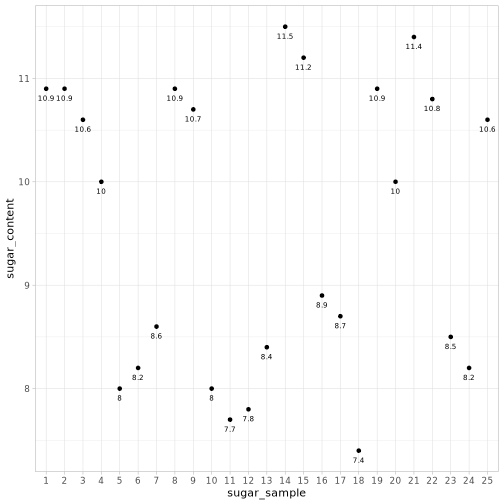
\includegraphics{hw_stat572_files/figure-latex/unnamed-chunk-1-1} \end{center}

(c). Give a specific example of an application where an Exponential
model would be reasonable. Give an example where an Exponential model
would NOT be appropriate, and explain why.

\hypertarget{a-poisson-case}{%
\subsubsection{2 A Poisson Case}\label{a-poisson-case}}

An ecologist records the number of eggs laid in a sample of sparrow
nests of size \(n=20\). Let \(Y_i\) be the number of eggs laid in nest i
for \(i=1,...,20\). Based on this sample, the ecologist is interested in
estimating \(\theta\), the mean number of eggs per nest in the general
population of nests. Assume \(Y_1,...,Y_n|\theta\sim Poisson(\theta)\)
iid, and also for now that \(\theta\in\Theta=\{0.1,0.2,...,4.9,5.0\}\)
and that \(p(\theta) = 1/50\) for each \(\theta\in\Theta\).

(a). Let \(X=\sum_i Y_i\) denote the random variable that counts the
total number of eggs laid in the 20 nests. Using the form of Bayes rule
on page 15 of the Hoff book, write down a formula for \(p(\theta|x)\)
and simplify as much as possible.

(b). The ecologist observes that \(x = 36\). Make a plot of
\(p(\theta|x)\) versus \(\theta\) for\(\theta\in\Theta\)

(c). Find \(E[\theta|x]\), the posterior mean of \(\theta\).

(d). Find two numbers, \(\theta_l\) and \(\theta_h\) such that
\(Pr(\theta_l\le\theta\le\theta_h|x)\approx 0.95\). This is an
approximate 95\% posterior confidence interval. Note that there is more
than one way of doing this.

(e). Remake the plot in part (b) but with \(n = 40\) and \(x = 72\).
Describe and explain the differences you see between this plot and the
one in (b).

\hypertarget{posterior-predictive-density}{%
\subsubsection{3 posterior predictive
density}\label{posterior-predictive-density}}

Suppose the data \(y_{1:n}|\theta\) is modeled as iid \(Exp(\theta)\),
and the prior is

\(p(\theta) = Gamma(\theta|a,b) = \frac{b^a}{\Gamma(a)} \theta^{a-1}e^{-b\theta}1_{\{\theta>0\}}\)

From problem 1, we know that the posterior is
\(p(\theta|y_{1:n}) = Gamma(\theta|a_n,b_n)\), where \(a_n=a+n\) and
\(b_n=b+\sum^n_{i=1} y_i\). What is the posterior predictive density
\(p(y_{n+1}|y_{1:n})\)? Give your answer as a closed-form expression
(not an integral).

\(p(y_{n+1}| y)\;=\; p(y_{n+1}| y_{1:n})=\int_{\theta\in\Theta} p(y_{n+1},\theta | y_{1:n}) d\theta\)
\(= \int_{\theta\in\Theta} p(y_{n+1} | \theta, y_{1:n}) p(\theta | y_{1:n}) d\theta\)
\(= \int_{\theta\in\Theta} p(y_{n+1} | \theta) p(\theta | y_{1:n}) d\theta\)

\(= \int_{\theta\in\Theta} \theta e^{-\theta y_{n+1}} \frac{(b+\sum y_i)^{a+n}}{\Gamma(a+n)}\theta^{a+n-1}e^{-(b+\sum y_i)\theta} d\theta\)

\(= \frac{(a+n)(b+\sum y_i)^{a+n}}{(b+\sum y_i+y_{n+1})^{a+n+1}} \int_{\theta\in\Theta} \frac{(b+\sum y_i+y_{n+1})^{a+n+1}}{\Gamma(a+n+1)}\theta^{a+n}e^{-(b+\sum y_i+y_{n+1})\theta}d\theta\)

\(= \frac{(a+n)(b+\sum y_i)^{a+n}}{(b+\sum y_i+y_{n+1})^{a+n+1}}\)

\hypertarget{decision-theory}{%
\subsubsection{4 (decision theory)}\label{decision-theory}}

Suppose that in the small imaginary city of our class example, where the
prevalence of a rare disease was studied (Foundations: Section 4, page
11), public health officials need to decide the amount of resources to
allocate towards prevention and treatment of the disease we are
concerned with, with the fraction of infected individuals \(\theta\)
still unknown. They will decide on the resources needed based on a
fraction \(c\) of the population. If \(c\) is chosen too large, there
will be wasted resources, while if it is too small, preventable cases
may occur and some individuals may go untreated. After some
deliberation, they tentatively adopt the following loss function:

\(\ell(\theta,c)=(\theta-c + 0.5)^2\) for \(c\in[0,1]\)

(a). Assume that the number of people sampled is again \(n=20\), that
\(y=0\), and use \(\theta\sim Beta(2,20)\) as the prior again to derive
the posterior expected loss.

\[p(\theta| y) \propto p(y| \theta) p(\theta)
=  {20 \choose y}\theta^y (1-\theta)^{20-y}\frac{1}{B(2,20)} \theta^{2-1} (1-\theta)^{20-1}\\
\propto \theta^{2+0-1} (1-\theta)^{20+(20-0)-1}
\propto \text{Beta}(2,40)\]

\[E(\boldsymbol{\theta}| Y=0)=\frac{a+0}{(a+0)+(b+n-0)}=\frac{2}{42}\]

Let \(\hat{\theta}=c-0.5\),
\(\ell(\theta,c)=(\theta-c + 0.5)^2=\theta^2-2\theta \hat{\theta}+\hat{\theta}^2\),

\(\rho(\hat{\theta},y_{1:n}) = E(\ell(\boldsymbol{\theta},\hat{\theta})| y_{1:n})= E(\boldsymbol{\theta}^2| y_{1:n})-2E(\boldsymbol{\theta}| y_{1:n}) \hat{\theta} + \hat{\theta}^2\)

\(= E(\boldsymbol{\theta}^2| y_{1:n})-2E(\boldsymbol{\theta}| y_{1:n})(c-0.5) +(c-0.5)^2\)

(b). Find an optimal value (call it \(\hat c\)) for \(c\) following a
Bayesian decision procedure using the set up from part (a).

\(\frac{d}{d\hat{\theta}}\rho(\hat{\theta},y_{1:n})=-2E(\boldsymbol{\theta}|y_{1:n})+2\hat{\theta}=0\)

\(\hat{\theta}=\delta(y_{1:n}) =E(\boldsymbol{\theta}|y_{1:n})=\frac{2}{42}=c-0.5\implies \hat c=\frac{23}{42}\)

(c). Graphically compare \(l(\theta,\hat c)\) and \(l(\theta,\bar y)\)
as \(\theta\) ranges from 0 to 1.

\begin{center}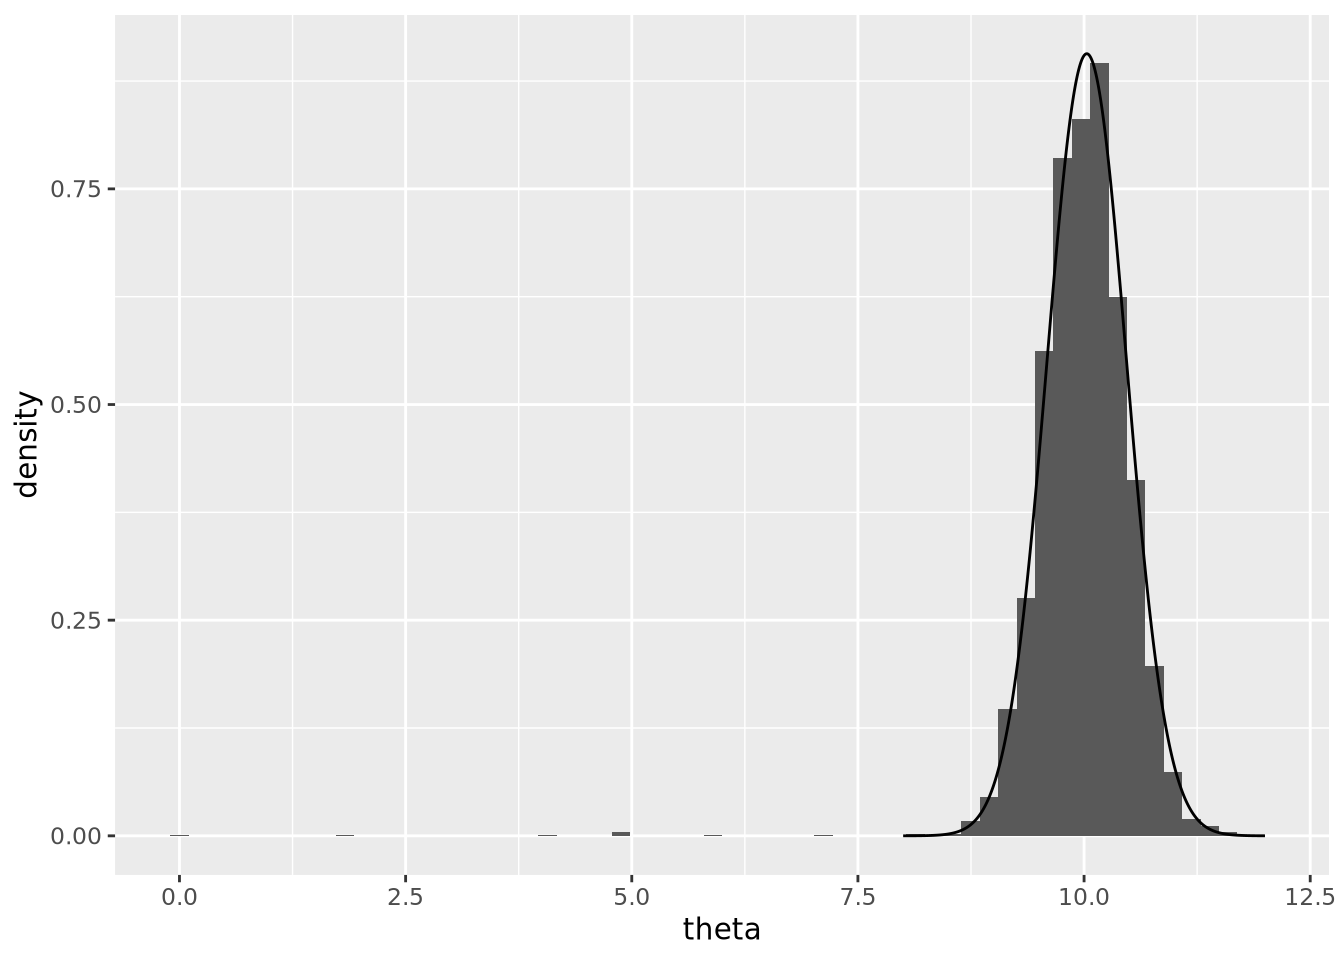
\includegraphics{hw_stat572_files/figure-latex/unnamed-chunk-6-1} \end{center}

(d). Compare the outcome from the Bayesian decision procedure to the
procedures that choose (i) \(c=\bar y\) and (ii) \(c=0.1\) constant
(i.e., setting it to the prior mean). This comparison can be done by
observing the optimal quantity \(c\) derived from each of the decision
procedures considered while varying the value of \(y\) (the number of
infected cases).

\begin{center}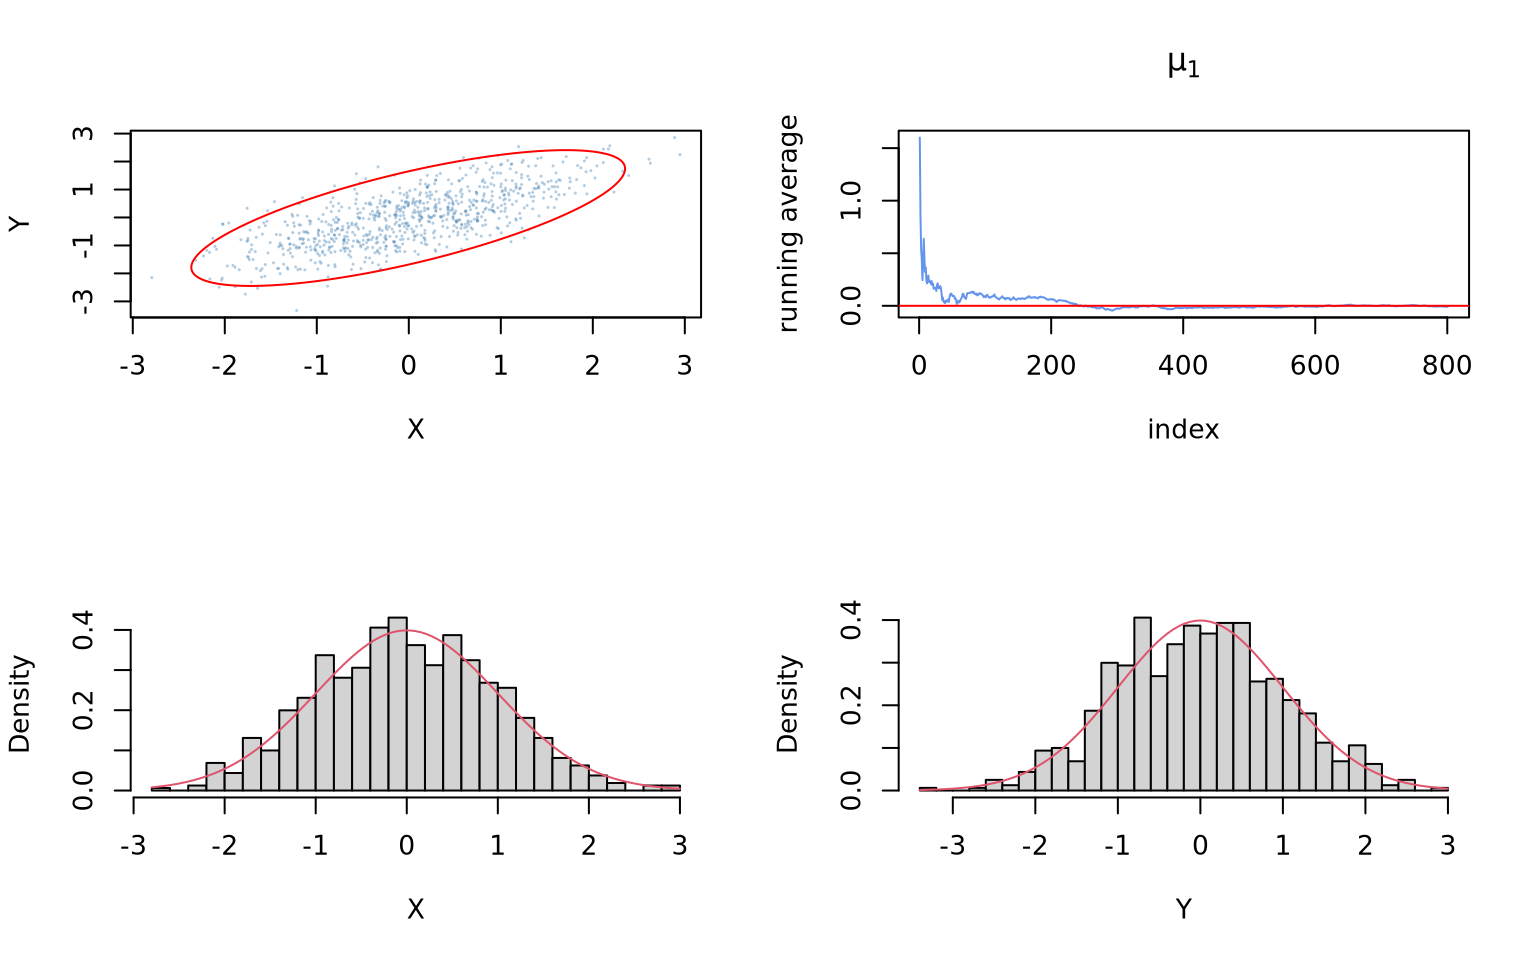
\includegraphics{hw_stat572_files/figure-latex/unnamed-chunk-7-1} \end{center}


\end{document}
